\subsection{Il metodo sqale}
A partire dalla sua pubblicazione, risalente al 2010, SQALE è diventato il metodo standard a livello industriale per la gestione del Technical Debt. Gli obiettivi principali di tale metodo sono sostanzialmente i seguenti:
\begin{enumerate}
	\item fornire una stima del costo del technical debt di un pezzo di codice sorgente;
	\item fornire indicatori che consentano un'analisi  dettagliata della natura del debito tecnico;
	\item supportare strategie di rimedio utilizzando indicatori. Esistono molte strategie potenziali e la scelta è dettata dal contesto;
	\item essere implementabili all'interno di una soluzione automatizzata per fornire supporto decisionale in tempo reale.
\end{enumerate}
Al fine di raggiungere tali obiettivi, il metodo SQALE utilizza quattro concetti:
\begin{enumerate}
	\item un modello di qualità;
	\item modelli di stima;
	\item indici;
	\item indicatori.
\end{enumerate}
\subsection{Il modello di qualità}
Il modello di qualità è una lista dei buoni principi che un team o un'organizzazione deve considerare per la definizione di un codice di qualità. Tale lista serve come riferimento per stimare il technical debt del codice. Qualsiasi non conformità con il modello di qualità crea debito e non vi è alcun debito senza la violazione di almeno uno dei requisiti. Se un'organizzazione non vuole definire una lista di questo tipo, oppure non ha a disposizione tempo sufficiente, può utilizzare modello noto come A2DAM (Agile Alliance Debt Analysis Model) oppure l'elenco predefinito fornito dagli strumenti di analisi statica.
\subsection{Modello di stima}
Il metodo SQALE contiene due modelli di stima. Il primo viene utilizzato per stimare il tempo necessario a rimediare ad ogni debito associato ad ogni item all'interno del codice. Si parla di \textit{remediation cost}. Il secondo modello stima l'impatto del debt sul business e si parla di \textit{non-remediation cost}. Esso stima i costi addizionali futuri e  potrebbe anche essere considerato come il costo legato al ritardare la risoluzione di un problema.
Pertanto, con SQALE, ogni voce di debito ha due costi:
\begin{itemize}
	\item il costo di riparazione,
	\item il costo di non riparazione.
\end{itemize}
Tutti questi calcoli sono eseguiti dagli strumenti di analisi che supportano il metodo.
La maggior parte di questi strumenti ha tali modelli di stima già preconfigurati, quindi è possibile iniziare ad analizzare il codice con le impostazioni predefinite.
Quando si aggiungono tutti i costi di riparazione di tutti gli elementi di debito rilevati dall'analisi del codice, si ottiene il debito tecnico del componente, dell'applicazione o del dominio software. Quando si aggiungono tutti i costi di non rimedio di un componente software, si ottiene l'impatto sul business (la parte di interesse) del componente.
\subsection{Indici}
Gli indici considerati sono due e derivano dai due modelli di stima. In particolare, si considerano:
\begin{itemize}
	\item technical debt index,
	\item business impact index.
\end{itemize}
Questi due indicatori dovrebbero essere monitorati e resi trasparenti a tutti i partecipanti a un progetto in modo tale che ognuno in ogni momento saprà quanto debito tecnico il progetto sta affrontando in termini di capitale o interesse. \\ Un altro indice importante è il debt ratio che è il debito tecnico diviso per il budget del progetto. Per tornare alla metafora finanziaria, un modo per valutare lo stato di salute di un'azienda è calcolare il suo rapporto di indebitamento, che è il rapporto tra i debiti e le attività della società. Per analogia, il rapporto di indebitamento SQALE consente di monitorare lo stato di salute dei progetti e delle applicazioni.
\subsection{Indicatori}
L'indicatore maggiormente utilizzato è lo SQALE rating. Sostanzialmente si associa una lettera a determinate percentuali di debt ratio. In particolare, le lettere vanno da A ad E e ad ogni lettera è associato un colore. Si mostra un esempio in \autoref{fig:rating}. Un debt ratio basso produce come risultato A, mentre il grado più alto è E.
\begin{figure}[htbp]
	\centering
	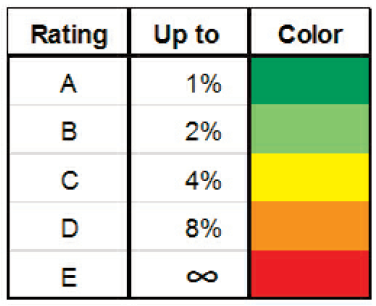
\includegraphics[scale=1, trim = 0cm 0cm 0cm 0cm, clip=true]{figSonarCloud/SQUALE1.png}
	\caption{Esempio di griglia del SQALE RATING}
	\label{fig:rating}
\end{figure}
Il secondo indicatore più utilizzato è la piramide SQALE, che rappresenta la distribuzione del debito tecnico in termini di caratteristiche di qualità come mostrato in \author{fig:piramide}. Questo indicatore può essere letto in due modi:
\begin{enumerate}
	\item  La vista analitica (rappresentata dai numeri nella colonna di sinistra e dalle barre di colore azzurro)
	\item La vista consolidata (rappresentata dai numeri nella colonna destra e dalle barre blu scuro)
\end{enumerate}

\begin{figure}[htbp]
	\centering
	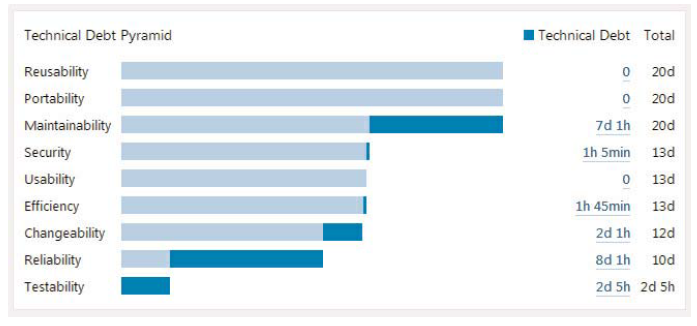
\includegraphics[scale=1, trim = 0cm 0cm 0cm 0cm, clip=true]{figSonarCloud/piramide.PNG}
	\caption{La piramide SQALE}
	\label{fig:piramide}
\end{figure}
La vista consolidata della piramide, si ottiene sommando il debito di tutti i livelli caratteristici inferiori per una data caratteristica.
Questi calcoli sono indicati dai numeri nelle colonne di destra. Si prenda ad esempio l'utilità,che ha un debito tecnico di 12 giorni. I progetti agili generano un numero elevato di cicli di modifica del codice. Le caratteristiche qualitative necessarie per supportare questi sviluppi sono la testabilità, l'affidabilità e la variabilità.
Poiché la variabilità si basa sull'affidabilità e sulla testabilità, la distanza reale tra lo stato corrente del codice e lo stato di destinazione del codice facilmente modificabile è la somma del debito associato a ciascuna delle tre caratteristiche (2d 5h + 8d 1h + 2d 1h = 12d). Questo valore consolidato risponde alla seguente domanda di un rappresentante aziendale: "Quanto siamo lontani dall'avere software modificabile?" Questo meccanismo di consolidamento è applicabile a tutte le caratteristiche
Altro indicatore SQALE è la mappa del debito SQALE. Si tratta di un grafico a bolle su cui un l'item (un file, un componente, un'applicazione) è rappresentato su due assi, il debito tecnico e l'impatto sul business, come mostrato in \autoref{fig:bolle}. 
\begin{figure}[htbp]
	\centering
	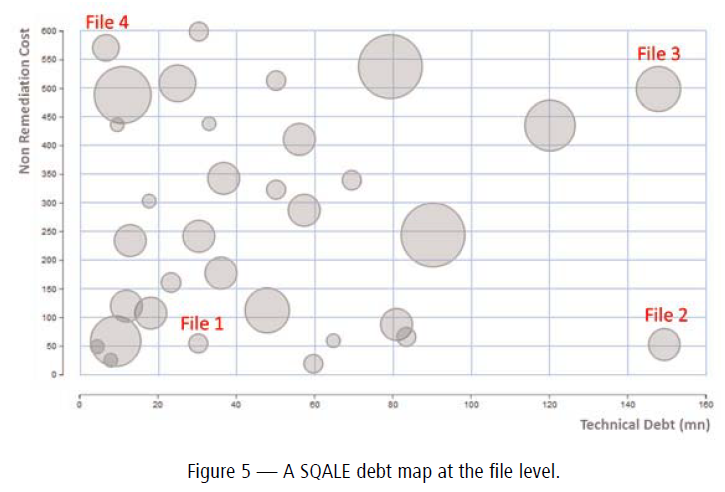
\includegraphics[scale=1, trim = 0cm 0cm 0cm 0cm, clip=true]{figSonarCloud/bolle.PNG}
	\caption{La piramide SQALE}
	\label{fig:bolle}
\end{figure}